%% SECTION HEADER /////////////////////////////////////////////////////////////////////////////////////
\section{Results of \acl{hsc} validation with \aclp{pzt} wave acquisition setup}
\label{sec:resuls_pzt}
%% SECTION CONTENT ////////////////////////////////////////////////////////////////////////////////////
Validation of the honeycomb structure models and a separate \ac{cfrp} plate intended for \ac{hsc} sample were done by comparing the group velocity and amplitude of the first packet of \ac{s0} and \ac{a0} arriving at the sensor.
Figure~\ref{fig:signal_exp_raw} contains examples of the experimentally obtained raw signals for the healthy and damaged samples.
The raw signals were processed for noise reduction and next an envelope of the signals was calculated.
The envelope was used to obtain the amplitude and group velocity of the mods for the model validation and was used in the analytical assessment of damage magnitude.
\begin{figure}[!htb]
	\begin{center}
		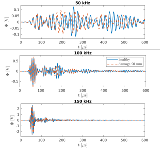
\includegraphics[width=0.95\textwidth]{Chapter_6/signal_exp_raw}
	\end{center}
	\caption{Raw signals registered by the sensor in \acl{hsc} for the specimen at healthy (solid line) and the damaged state - disbonds width of 90 \unit{\mm} (dashed line)}
	\label{fig:signal_exp_raw}
\end{figure}
\pagebreak

Signal processing followed the diagram shown in Figure~\ref{fig:signal_processing}.
A preliminary step was a conversion of the signals from the time domain to the frequency domain by the \ac{fft}.
Then, the band-pass filter was applied in the range \(0.5f_c-1.5f_c\).
For this purpose a Butterworth filter of 20th order was used.
After filtering, the signal was converted back to the time domain by the \ac{ifft}.
Lastly, the envelope of the signal \(e(t)\) was obtained using Eq. (\ref{eq:envelope}).

\begin{figure}[!htb]
	\begin{center}
		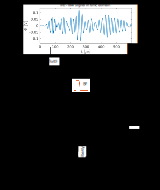
\includegraphics[width=0.95\textwidth]{Chapter_6/signal_processing}
	\end{center}
	\caption{Raw signals registered by the sensor in \acl{hsc} for healthy state and damage of 90 \unit{\mm} width}
	\label{fig:signal_processing}
\end{figure}

The group velocity was derived from the signal envelope related to particular Lamb wave mode and its \ac{tof}.
The \ac{tof} is a difference between the arrival of the maximum amplitude of the envelope of considered mode at the sensor \((\mathrm{T}_1)\) and the half time of the excitation pulse \(\left(\mathrm{T}_0=0.5/f_m\right)\).
Since the distance between the transducers was constant \(l=200\) \unit{\mm}, the group velocity equals
\begin{eqnarray}
	C_g = \frac{\mathrm{ToF}}{l}=\frac{T_1-T_0}{l}.
\end{eqnarray}

The signal envelopes are shown in Figure~\ref{fig:single_skin} for single \ac{cfrp} plate, Figure~\ref{fig:hsc_full} for the \ac{fcgm}, and Figure~\ref{fig:hsc_homo}, from which the velocities and amplitudes of the wave mods were determined.
\begin{figure}[!htb]
	\begin{center}
		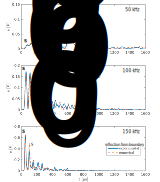
\includegraphics[width=0.95\textwidth]{Chapter_6/single_skin}
	\end{center}
	\caption{The signal envelope for single \acs{cfrp} skin; experimental vs. numerical simulation}
	\label{fig:single_skin}
\end{figure}

For the single \ac{cfrp} plate, Table~\ref{tab:group_velocity_cfrp} gives the determined velocities and amplitudes of the modes together with the percentage errors defined by
\begin{eqnarray}
	\delta = \left|\frac{x^{num}-x^{exp}}{x^{exp}}\right|\times100\%,
	\label{eq:perc_err}
	\nomtypeG[delta]{\(\delta\)}{Percentage error}{}{\%}%
\end{eqnarray}
where \(x^{num}\) and \(x^{exp}\) are the numerical and experimental values, respectively.
It can be noticed that the model is in good agreement with experimental results.
All values are within an error of up to 10\%, except for the \ac{s0} and \ac{a0} amplitudes for 50 and 100 \unit{\kHz}, respectively.
For these cases, the error is about 25\%.
The \ac{a0} mode at 150 \unit{\kHz} in Figure~\ref{fig:hsc_homo} was not identified because the high amplitude \ac{s0} reflections mask it.

Regarding \ac{hsc} panel, the best results were achieved for the \ac{fcgm} as it is shown in Table~\ref{tab:group_velocity_hsc}.
The velocity error is less than 10\% for both modes except for the signal at 50 \unit{\kHz}. 
In the case of signals amplitude, the simulation results are underestimated.
Only the \ac{s0} at 100 and 150 \unit{\kHz} has the error less than 15\%.
For the \ac{hcgm}, the best result were obtained for the \ac{s0} at 150 \unit{\kHz} with error less than 11\%.
Amplitudes of the \ac{a0} for this model are more accurate than the \ac{fcgm} with the errors below 15\%.
\begin{figure}[!htb]
	\begin{center}
		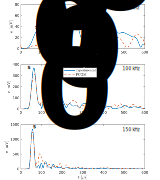
\includegraphics[width=0.95\textwidth]{Chapter_6/HSC_full}
	\end{center}
	\caption{The signal envelope for the \acl{hsc} structure; experimental vs. the \acf{fcgm}}
	\label{fig:hsc_full}
\end{figure}

\begin{figure}[!htb]
	\begin{center}
		\includegraphics[width=0.95\textwidth]{Chapter_6/HSC_homo}
	\end{center}
	\caption{The signal envelope for the \acl{hsc} structure; experimental vs. the \acf{hcgm}}
	\label{fig:hsc_homo}
\end{figure}
\begin{table}[!htb]
	\small
	\tabcolsep=0.2cm
	\centering
	\caption{\label{tab:group_velocity_cfrp} Comparison between amplitudes and group velocities obtained from the simulations and experiments for the single \acs{cfrp} plate}
	\begin{tabular}{cccccccc}
		\toprule
		& & \multicolumn{3}{c}{\(C_g\)} & \multicolumn{3}{c}{Amp.}\\
		Mode & Frequency & Exp. & Num. & \(\delta\)& Exp. & Num. & \(\delta\)\\
		& \unit{\kHz} & \unit[per-mode = symbol]{\m\per\s} & \unit[per-mode = symbol]{\m\per\s} & \% & \unit{\mV} & \unit{\mV} & \% \\
		\midrule
		\multirow{3}{*}{\ac{s0}} & 50 & 6079 & 5865 & \textcolor{green}{3.52}& 12 & 171 & \textcolor{red}{25.0} \\
		&100& 5571 & 5747 & \textcolor{green}{3.16} & 171 & 162 & \textcolor{green}{5.26}\\
		&150& 5764 & 5698 & \textcolor{green}{1.15} & 648 & 664 & \textcolor{green}{2.47}\\
		\midrule
		\multirow{3}{*}{\ac{a0}} &50& 1341 & 1325 & \textcolor{green}{0.74} & 134 & 125 & \textcolor{green}{6.72}\\
		&100& 1550 & 1396 & \textcolor{green}{9.74} & 84 & 104 & \textcolor{red}{23.8}\\
		\bottomrule
	\end{tabular}
\end{table}

Errors in the models may be due to several factors.
The most important ones include differences in material properties of used components.
In the models, an average thickness of the adhesive layer was assumed; obtaining precise thickness of the adhesive layer in the specimen preparation is difficult under workshop conditions.
The models also assumed the same shape for each core cell, whereas in practice, the geometry was different because of in-plane deformation of the core during the sample preparation.
The velocity in the panel varies with the angle of propagation due to anisotropy of \ac{cfrp} plate and the geometry of the honeycomb core.
In the models, the direction of wave propagation between the sensors was assumed to coincide with the skin and core orientation.
\clearpage


\begin{table}[!htb]
	\small
	\tabcolsep=0.15cm
	\centering
	\caption{\label{tab:group_velocity_hsc} Comparison between amplitudes and group velocities obtained from the simulations based on the \acf{fcgm} and the \acf{hcgm} and experiments for \acl{hsc}}
	\begin{tabular}{cccccccccccc}
		\toprule
		& & \multicolumn{5}{c}{\(C_g\)} & \multicolumn{5}{c}{Amp.}\\
		Mode & Freq.& Exp. & \ac{fcgm} & \(\delta\) & \ac{hcgm} & \(\delta\) &  Exp. & \ac{fcgm} & \(\delta\) & \ac{hcgm} & \(\delta\)\\
		& \unit{\kHz} & \unit[per-mode = symbol]{\m\per\s} & \unit[per-mode = symbol]{\m\per\s} & \% & \unit[per-mode = symbol]{\m\per\s} & \% & \unit{\mV} & \unit{\mV} & \%& \unit{\mV} & \% \\
		\midrule
		\multirow{3}{*}{\ac{s0}} & 50 & 6452 & 8696 & {34.78} & 8333 & {29.15} & 32 & 6 & \textcolor{red}{81.25} & 3 & \textcolor{red}{90.63}\\
		&100& 5263 & 5128 & \textcolor{green}{2.57} & 5714 & \textcolor{green}{8.57} & 369 & 314 & \textcolor{green}{14.91} & 138 & \textcolor{red}{62.6}\\
		&150& 5085 & 5217 & \textcolor{green}{2.60} & 4959 & \textcolor{green}{2.48} & 1341 & 1239 & \textcolor{green}{7.61} & 1482 & \textcolor{green}{10.51}\\
		\midrule
		\multirow{3}{*}{\ac{a0}} & 50 & 966 & 926 & \textcolor{green}{4.14} & 1316 & {36.23} & 62 & 76 & {22.58} & 63 & \textcolor{green}{1.61}\\
		& 100 & 2174 & 2151 & \textcolor{green}{1.06} & 2273 & \textcolor{green}{4.55} & 137 & 179 & {30.66} & 117 & \textcolor{green}{14.60}\\
		\bottomrule
	\end{tabular}
\end{table}